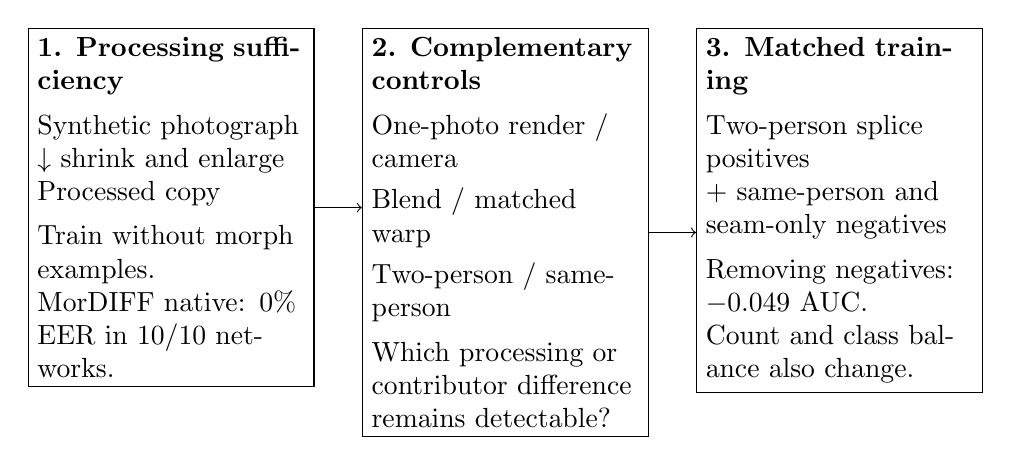
\begin{tikzpicture}
\node[draw,text width=.28\textwidth,align=left,anchor=north west] (a) at (0,0) {
\textbf{1. Processing sufficiency}\\[4pt]
Synthetic photograph\\
$\downarrow$ shrink and enlarge\\
Processed copy\\[4pt]
Train without morph examples.\\
MorDIFF native: 0\% EER in 10/10 networks.};
\node[draw,text width=.28\textwidth,align=left,anchor=north west] (b) at (.35\textwidth,0) {
\textbf{2. Complementary controls}\\[4pt]
One-photo render / camera\\[3pt]
Blend / matched warp\\[3pt]
Two-person / same-person\\[4pt]
Which processing or contributor difference remains detectable?};
\node[draw,text width=.28\textwidth,align=left,anchor=north west] (c) at (.70\textwidth,0) {
\textbf{3. Matched training}\\[4pt]
Two-person splice positives\\
$+$ same-person and seam-only negatives\\[4pt]
Removing negatives: $-0.049$ AUC.\\
Count and class balance also change.};
\draw[->] (a.east) -- (a.east -| b.west);
\draw[->] (b.east) -- (b.east -| c.west);
\end{tikzpicture}
